\chapter{Introduction to UNIX and Linux}
\label{chap:unix1}

% check out http://www.ibm.com/developerworks/aix/library/au-badunixhabits.html

\section{What is UNIX?}

UNIX is a machine-independent operating system (OS) developed in the 
1970s by AT\&T programmers (notably Brian Kernighan and Dennis Ritchie, 
fathers of {\tt C}) for programmers (you!). It is multi-user and 
network-oriented by design, uses plain text files for storing data (no 
proprietary file formats), and has a strictly hierarchical directory 
structure (more on this below). This makes it an ideal environment for 
developing your code and storing your data.

Linux and Mac OS are Unix-like (or UN*X or *nix) operating systems that 
have evolved from UNIX. Ubuntu is a Linux distribution.

\section{Why UNIX?}
Here are some good reasons:
 \begin{compactitem}
  \item It was designed for developing code and storing data --- 
  an ideal native habitat for programming languages like Python and R! 
  \item Robust, stable, secure (very few UNIX viruses and malware --- I have never encountered one!) 
  \item Free and open source!
  \item Scores of small programs available to perform simple tasks -- can be 
combined easily
  \item Easy to automate tasks (e.g., using shell scripts)
  \item Multi-user (multiple users can log in concurrently use computer)
  \item Multi-tasking (can perform many tasks at the same time)
  \item Network-ready (easy to communicate between computers)
  \item UNIX has been around since the early 1970's and will likely be 
  around at the end of your career (the hard work you are putting into 
  learning UNIX will pay off over a lifetime!)
  \item Amazing support --- a large body of tutorials and support web 
  sites are readily available online. 
	\item Basically all resources for High-Performance Computing (computer clusters, large workstations, etc.) run a
UNIX or Linux operating system. 
  \end{compactitem}

See \url{http://whylinuxisbetter.net/} (I would have chosen a more 
subtle domain name though!) to aid your brain-washing (cleaning?).

Also, if you like history: {\sloppy \url{https://www.howtogeek.com/182649/htg-explains-what-is-unix}}

\begin{tipbox}
The terms 32-bit and 64-bit refer to the way a computer's processor (also called a CPU), handles information. A 64-bit OS handles large amounts of random access memory (RAM) more effectively than a 32-bit system. Specifically, while 32 bits of information can only access 4 GB of RAM, a 64-bit machine can access essentially unlimited system memory (though this is not yet physically possible)!  
\end{tipbox}  

\section{UNIX directory structure}

\begin{center}
  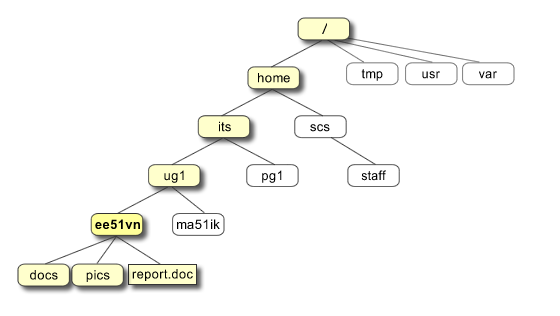
\includegraphics[width=.7\textwidth]{unix-tree.png}\\
  \url{ https://pathanruet.files.wordpress.com/2012/05/unix-tree.png}	
\end{center}

The UNIX directory (same as ``Folder'') structure is hierarchical, with 
a single tree starting from the ``root'' {\tt /}. This is quite unlike 
Windows or MS-DOS, where there are separate trees for disk partitions, 
removable media, network, etc. The key UNIX directories are:
 
\begin{tabular}{p{2cm} p{10cm}} 
 {\tt /} & Is the "root" directory\\
 {\tt /bin} & Contains basic programs\\
 {\tt /etc} & Contains configuration files\\
 {\tt /dev} & Contains files connecting to devices (keyboard,
  mouse, screen, etc.)\\
 {\tt /home} & Your home directory -- this is where you will usually work\\
 {\tt /tmp} & Contains Temporary files\\
\end{tabular}

This hierarchical directory structure makes navigating your 
computer from the terminal/shell (coming up next!) or encoding this 
navigation in your computer programs easier. 

\begin{tipbox}
When you install Linux (say, a Ubuntu version), you will have the opportunity to create separate {\tt swap}, {\tt root} and {\tt home} partitions on your hard disk. {\tt swap} necessarily needs to be a separate partition, while  {\tt root + home} can be on the same partition. If you are a Linux newbie, I suggest that you create a separate {\tt home} partition, even though it is not necessary --- that way, even if you break your linux install, you can easily reinstall it by just wiping the root partition, without losing any of your data (which sits in {\tt home}).  
% In general, you should be fine with a root - only partition between 2GB and 8GB.
\end{tipbox}
  
\section{Meet the UNIX shell}

The shell (or terminal) is a text command processor to interface with 
the Operating System's ``kernel''. We will use the popular (yes, it's 
popular!) {\tt bash} shell. 

\begin{compactitem}[$\quad\star$]\itemsep4pt
	\item To launch {\tt bash} shell, do {\tt Ctrl + Alt + t} (or use {\tt 
Meta} key) --- try it now.
\end{compactitem}

OK, so you have met the shell. Note that:
\begin{compactitem}
   \item The shell automatically starts in your home directory 
  {\tt /home/yourname/}, also called $\sim$ (important to remember!)
   \item Use the {\tt Tab} key -- very handy (try {\tt ls} with {\tt Tab} 
{\tt Tab})
   \item You can navigate commands you previously typed using the up/down arrows  
\end{compactitem}

Other useful keyboard shortcuts are:

\begin{tabular}{p{4.4cm} p{9cm}} 
  {\tt Ctrl + A} & Go to the beginning of the line\\
  {\tt Ctrl + E} & Go to the end of the line\\
  {\tt Ctrl + L} & Clear the screen\\
  {\tt Ctrl + U} & Clear the line before cursor position\\
  {\tt Ctrl + K} & Clear the line after the cursor\\
  {\tt Ctrl + C} & Kill whatever you are running\\
  {\tt Ctrl + D} & Exit the current shell\\
  {\tt Ctrl + right arrow} & Move cursor forward one word\\
  {\tt Ctrl + left arrow} & Move cursor backward one word\\
  \end{tabular}

\section{{\tt sudo}, and installing/removing software}

You can install software in your {\tt /home} directory. In UNIX you 
originally had to login as {\tt root} (administrator). But in Ubuntu, 
it is sufficient to add {\tt sudo} ({\tt s}uper {\tt u}ser {\tt do}) in 
front of a command: 
\begin{lstlisting}
sudo apt-get install geany geany-plugins geany-plugin-latex 
geany-plugin-addons
\end{lstlisting}

You can install anything that is in the Ubuntu "repository". Let's try 
installing something else --- a weather indicator that I think really works
very well. 

But here you have to first install the repository: 
\begin{lstlisting}
$ sudo add-apt-repository ppa:atareao/atareao
\end{lstlisting}

This will ask you to first approve the additon of this repository. Then 
update the repository packages, 
\begin{lstlisting}
$ sudo apt-get update 
\end{lstlisting}

And then install,
\begin{lstlisting}
$ sudo apt-get install my-weather-indicator
\end{lstlisting}

\begin{center}
	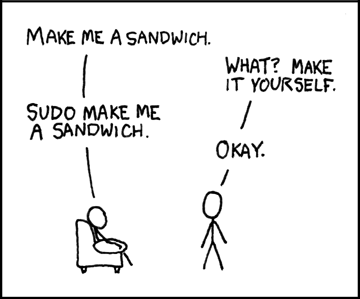
\includegraphics[width = 0.4\linewidth]{sandwich.png}\\
	{\tt http://xkcd.com/149/}
\end{center}					

You can also easily remove software by, well, using the {\tt remove} 
command! You will find that commands names are quite intuitive, as they 
should be. If you think a command with a certain name should exist, it 
very often does!

\begin{lstlisting}
$ sudo apt-get remove indicator-messages
\end{lstlisting}

This will get rid of the evolution mail indicator --- very unlikely 
that you will use evolution!

\section{Basic UNIX commands}
 
\begin{tabular}{p{.3\textwidth} p{.7\textwidth}} 
 {\tt man [COMMAND]} & Show help page of a command.\\
 {\tt whoami} & Display your user-name.\\
 {\tt pwd} & Show the current directory.\\
 {\tt ls} & List the files in the directory.\\
 {\tt cd [DIRNAME]} & Change directory.\\ 
 {\tt cd ..} & Move one directory up. \\
 {\tt cd /} & Go to the root directory. \\
 {\tt cd $\sim$} or just {\tt cd } & Go to the home directory.\\
 {\tt cp [FROM] [TO]} & Copy a file or directory non-recursively (what's this?).\\
 {\tt mv [FROM] [TO]} & Move or rename a file or directory.\\
 {\tt touch [FILENAME]} & Create an empty file.\\
 {\tt echo "My string"} & Print a string (here, "My string").\\
 {\tt rm [TOREMOVE]} & Remove a file or directory non-recursively.\\
 {\tt mkdir [DIRNAME]} & Create a directory.\\
 {\tt rmdir [DIRNAME]} & Remove an empty directory.\\
 {\tt wc [FILENAME]} & Count the number of lines and words in a file.\\
 {\tt sort [FILENAME]} & Sort the lines of a file and print result.\\
 {\tt uniq } & Shows only unique elements of a list.\\
 {\tt cat [FILENAME]} & Print the file on the screen.\\
 {\tt less [FILENAME]} & Progressively print a file on the screen ("q" 
 to exit).\\
 {\tt head [FILENAME]} & Print the first few lines of a file.\\
 {\tt tail [FILENAME]} & Print the last few lines of a file.\\
 {\tt history} & Show the last commands you typed.\\
 {\tt date} & Print current date.\\
 {\tt file [FILENAME]} & Determine the type of a file.\\
 {\tt passwd} & Change user password.\\
 {\tt chmod [FILENAME]} & Change file permissions.
\end{tabular}
  
\section{Building your coursework directory structure}

It is time to start building your CMEE coursework directory structure. 
Please follow these rules:
	\begin{compactitem}

		\item Do all your work in {\tt CMEECourseWork}, located in a 
		suitable place in your {\tt /home} (make mama proud, keep your {\tt 
		home} organized!)
	 \item Each week's coursework should be in its respective directory: 
	 {\tt CMEECourseWork/Week1}, {\tt CMEECourseWork/Week2}, etc
	 \item Each week's directory will contain directories called {\tt 
	 Code}, {\tt Data}, etc (later)
		\item You will bring {\tt CMEECourseWork} and all it's contents 
			 under version control using Git (later)
  \end{compactitem}

\begin{tipbox}
Don't forget to use the {\tt tab} key. It autocompletes directory 
names for you (same in {\tt R} and {\tt Python}, and/or provides  
a list of files in the current directory (hit {\tt tab} twice after 
certain commands. For example, try double tab after typing {\tt ls} 
at the bash prompt.)  	
\end{tipbox}

\begin{compactitem}[$\quad\star$]\itemsep4pt
	\item OK, {\tt mkdir} your {\tt CMEECourseWork} directory now.
\end{compactitem}
Starting by creating {\tt CMEECourseWork}). Then,

\begin{lstlisting}
$ mkdir Week1
$ cd Week1
$ mkdir sandbox
$ cd Sandbox
bash: cd: Sandbox: No such file or directory
$ cd ..
$ rm sandbox
rm: cannot remove `sandbox/`: Is a directory
$ mv sandbox Sandbox # OR, "rm -r sandbox" (careful with the -r option!)
\end{lstlisting}

Note the hash mark \# above --- anything after a \# is ignored (so you 
can use it for commenting).

\begin{lstlisting}
$ cd Sandbox
$ pwd
$ ls
$ touch TestFile # OR, "touch TestFile.txt"
$ ls
$ mv TestFile TestFile2
$ rm TestFile2
\end{lstlisting}

You could have made your project directories and subdirectories in one 
swoop by using the {\tt -p} option of {\tt mkdir}: 

\begin{lstlisting}
$ mkdir -p CMEECourseWork/Week1/{Data,Code,Sandbox}
\end{lstlisting}

% Note: ``$\textbackslash$'' means multi-line code (can be entered verbatim
% in bash/terminal)
 
\section{Command arguments}

Most UNIX commands accept arguments that modify their behavior. E.g.,  {\tt ls 
-l} (ls ``minus''l) lists the files in longer format. Some useful 
arguments:
 
\begin{tabular}{p{.4\textwidth} p{.6\textwidth}} 

{\tt cp -r [DIR1] [DIR2]} & Copy a directory recursively (i.e., including 
all the sub-directories and files).\\
{\tt rm -i [FILENAME]} & Remove a file, but asks first (for safety).\\
{\tt rm -r [DIR]} & Remove a directory recursively (i.e., including all the 
sub-directories and files).\\
{\tt ls -a} & List all files, including hidden ones.\\
{\tt ls -h} & List all files, with human-readable sizes (Mb, Gb).\\
{\tt ls -l} & List all files, long format.\\
{\tt ls -S} & List all files, order by size.\\
{\tt ls -t} & List all files, order by modification time.\\
{\tt ls -1} & List all files, one file per line.\\
{\tt mkdir -p Dir1/Dir2/Dir3} & Create the directory Dir3 and Dir1 and 
Dir2 if they do not already exist.\\
{\tt sort -n} & Sort all the lines, but use numeric values
  instead of dictionary (i.e., 11 follows 2).\\
\end{tabular}

You can also combine command arguments. Try:
\begin{lstlisting}
$ ls -1t #combines -l and -t
\end{lstlisting}

\section{Redirection and pipes}

Output of programs can also be ``redirected'' to a file:

\begin{tabular}{p{.1\textwidth} p{.9\textwidth}} 
  {\tt >} & Redirect output from a command to a file on disk. If
    the file already exists, it will be overwritten.\\
  {$>>$} & Append the output from a command to a file on disk. If
    the file does not exist, it will be created.\\
\end{tabular}
 
Examples (make sure you are in {\tt Week1/Sandbox}):
      
\begin{lstlisting}
$ echo "My first line." > test.txt
$ cat test.txt
$ echo "My second line" >> test.txt
$ ls / >> ListRootDir.txt
$ cat ListRootDir.txt #Isn't that cool?!
\end{lstlisting}
 
We can also concatenate commands using ``pipes'' with ``$\vert$'' e.g., 
to count how many files are in root (/) directory:
\begin{lstlisting}
$ ls / | wc -l # what does this do? Look up "man wc"
\end{lstlisting}
Or try
\begin{lstlisting}
$ ls -lt | head -5 #what does this do?
\end{lstlisting}

\section{Wildcards}

We can use wildcards to find files based on their names (again, in 
{\tt Week1/Sandbox} !):
 
\begin{lstlisting}
$ mkdir TestWild
$ cd TestWild
$ touch File1txt
$ touch File2.txt
$ touch File3.txt
$ touch File4.txt
$ touch File1.csv
$ touch File2.csv
$ touch File3.csv
$ touch File4.csv
$ touch Anotherfile.csv
$ touch Anotherfile.txt
$ ls 
$ ls | wc -l
\end{lstlisting}

We will use the following wildcards:

\begin{tabular}{p{.2\textwidth} p{.8\textwidth}} 
  {\tt ?} & Any single character, except a leading dot (hidden 
  files).\\
  {\tt *} & Zero or more characters, except a leading dot (hidden 
  files).\\
	{\tt [A-Z]} & Define a class of characters (e.g., upper-case 
	letters).\\
\end{tabular}
 
Now let's try to find the files using wildcards:

\begin{lstlisting}
$ ls *
$ ls File*
$ ls *.txt
$ ls File?.txt
$ ls File[1-2].txt
$ ls File[!3].*
\end{lstlisting}

\section{Using {\tt grep}}

{\tt grep} is a command that matches strings in a file (why is this 
useful?). It is based on regular expressions (more on this later). 
Let's explore some basic usage of {\tt grep}. For a test file let's 
download a list of protected species from the UN website (to 
{\tt Sandbox}):
 
\begin{lstlisting}
$ wget http://www.cep.unep.org/pubs/legislation/spawannxs.txt #Cool!
$ head -n 50 spawannxs.txt #You will see "head" in R as well
\end{lstlisting}

Now,

\begin{lstlisting}
$ mkdir ../Data #Note the relative path "../"
$ mv spawannxs.txt ../Data/
$ cd ../Data
$ head -n 50 spawannxs.txt 
\end{lstlisting}

Note that now you have a {\tt Data} directory. 

OK, what about falcons? 
 
\begin{lstlisting}
$ grep Falco spawannxs.txt
Falconidae	Falco		femoralis septentrionalis
Falconidae	Falco		peregrinus
Falconidae	Polyborus	plancus
Falconidae	Falco		columbarius
\end{lstlisting}

Using {\tt -i} make the matching case-insensitive:
 
\begin{lstlisting}
$ grep -i Falco spawannxs.txt
Order:	FALCONIFORMES
Falconidae	Falco		femoralis septentrionalis
Falconidae	Falco		peregrinus
Falconidae	Polyborus	plancus
Order:	FALCONIFORMES
Order:	FALCONIFORMES
Order:	FALCONIFORMES
Falconidae	Falco		columbarius
\end{lstlisting}

Now let's find the beautiful ``Ara'' macaws:
\begin{center}
  
\includegraphics[width=.7\textwidth]{Ara_ararauna.jpg}
\end{center}

But this poses a problem (what is the problem?):

\begin{lstlisting}
$ grep -i ara spawannxs.txt
Flacourtiaceae	Banaras		vanderbiltii
Order:	CHARADRIIFORMES
Charadriidae	Charadrius	melodus
Psittacidae	Amazona		arausica
Psittacidae	Ara		macao
Dasyproctidae	Dasyprocta	guamara
Palmae		Syagrus (= Rhyticocos)	amara
Psittacidae	Ara		ararauna
Psittacidae	Ara		chloroptera
Psittacidae	Arao		manilata
Mustelidae	Eira		barbara
Order:	CHARADRIIFORMES
\end{lstlisting}

We can solve this by specifying {\tt -w} to match only full words:
 
\begin{lstlisting}
$ grep -i -w ara spawannxs.txt
Psittacidae	Ara		macao
Psittacidae	Ara		ararauna
Psittacidae	Ara		chloroptera
\end{lstlisting}

And also show line(s) after the one that was  matched, we can use {\tt 
-A x}, where {\tt x} is number of lines to use:

\begin{lstlisting}
$ grep -i -w -A 1 ara spawannxs.txt
Psittacidae	Ara		macao

--
Psittacidae	Ara		ararauna
Psittacidae	Ara		chloroptera
Psittacidae	Arao		manilata
\end{lstlisting}

Similarly, {\tt -B} shows the lines before:
 
\begin{lstlisting}
$ grep -i -w -B 1 ara spawannxs.txt
Psittacidae	Amazona		vittata
Psittacidae	Ara		macao
--
Psittacidae	Amazona		ochrocephala
Psittacidae	Ara		ararauna
Psittacidae	Ara		chloroptera
\end{lstlisting}

Use {\tt -n} to show the line number of the match:
 
\begin{lstlisting}
$ grep -i -w -n ara spawannxs.txt
216:Psittacidae	Ara		macao
461:Psittacidae	Ara		ararauna
462:Psittacidae	Ara		chloroptera
\end{lstlisting}

To print all the lines that do not match a pattern, use {\tt -v}:
 
\begin{lstlisting}
$ grep -i -w -v ara spawannxs.txt
\end{lstlisting}

To match one of several strings, use {\tt grep 
"string1$\backslash\vert$string2" file}. {\tt grep} can be used on 
multiple files, all files, using wildcards for filenames, etc -- 
explore as and when you need.

\section{Finding files with {\tt find}}

Its's easy to find files in UNIX using {\tt find}! Let's test it (make 
sure you are in {\tt Sandbox}, not {\tt Data}!)
 
\begin{lstlisting}
$ mkdir TestFind
$ cd TestFind
$ mkdir -p Dir1/Dir11/Dir111 #what does -p do?
$ mkdir Dir2
$ mkdir Dir3
$ touch Dir1/File1.txt
$ touch Dir1/File1.csv
$ touch Dir1/File1.tex
$ touch Dir2/File2.txt
$ touch Dir2/file2.csv
$ touch Dir2/File2.tex
$ touch Dir1/Dir11/Dir111/File111.txt
$ touch Dir3/File3.txt
\end{lstlisting}

Now find particular files:
 
\begin{lstlisting}
$ find . -name "File1.txt"
./Dir1/File1.txt
\end{lstlisting}

Using {\tt -iname} ignores case, and you can use wildcards:
 
\begin{lstlisting}
$ find . -iname "fi*.txt"
./Dir1/File1.txt
./Dir1/Dir11/Dir111/File111.txt
./Dir3/File3.txt
./Dir2/File2.txt
\end{lstlisting}

You can limit the search to exclude sub-directories:
 
\begin{lstlisting}
$ find . -maxdepth 2 -name "*.txt"
./Dir1/File1.txt
./Dir3/File3.txt
./Dir2/File2.txt
\end{lstlisting}

You can exclude certain files:
 
\begin{lstlisting}
$ find . -maxdepth 2 -not -name "*.txt"
.
./Dir1
./Dir1/File1.tex
./Dir1/File1.csv
./Dir1/Dir11
./Dir3
./Dir2
./Dir2/File2.tex
./Dir2/File2.csv
\end{lstlisting}

To find only directories:
 
\begin{lstlisting}
$ find . -type d
.
./Dir1
./Dir1/Dir11
./Dir1/Dir11/Dir111
./Dir3
./Dir2
\end{lstlisting}

\begin{tipbox}
There are are many ways in which you can tweak your Linux/UNIX 
environment and bash/terminal to your likes. For example, see 
\url{http://www.howtogeek.com/tag/ubuntu/ubuntu-tips/}.

But be careful, it can be addictive, and sometimes dangerous to your 
system's stability! 

Here are a couple of tweaks that I really find useful:\\

{\it Opening nautilus from terminal}

In terminal you can enter "f" to open nautilus in current directory 
by doing the following. Open your {\tt .bashrc} for editing:

\begin{lstlisting}
$ sudo gedit ~/.bashrc
\end{lstlisting}

Then add to the last line (type it, don't copy and paste!):\\
{\tt alias f='nautilus .'}

Then restart terminal or in current terminal:
\begin{lstlisting}
$ source ~/.bashrc
\end{lstlisting}

{\it Enabling autocomplete in terminal}

What happens when you use up and down keys in terminal? If nothing, 
then you need to enable reverse searching history. To do so, open 
{\tt /etc/inputrc}

\begin{lstlisting}
$ sudo geany /etc/inputrc
\end{lstlisting}

Then, add the following to it:

\begin{lstlisting}
## arrow up
"\e[A":history-search-backward
## arrow down
"\e[B":history-search-forward
\end{lstlisting}


Then close current terminal, open new one, and try up and down keys 
again.
\end{tipbox}
	      
\section[]{Practical: Make sure the basics work}
 
 \begin{enumerate} \itemsep10pt
		
		\item {\bf Some instructions}: 
		
		Review (especially if you got lost along the way) and make 
		sure you can run and understand all the commands and get the 
		expected outputs we have covered today. 
		
		Make sure you have your directory organized with {\tt Data} 
		and {\tt Sandbox} with the necessary files, under {\tt 
		CMEECourseWork/Week1}.

		Along with the completeness of the practicals/exercises 
		themselves, you will be marked on the basis of how complete and 
		well-organized your directory structure and content is -- in all 
		coming weeks as well.

	\item Here is a more complicated bash command using two pipes {\it you 
	are not expected to include the answer to this one as part of your 
	weekly submission}:
	
\begin{lstlisting}
$ find . -type f -exec ls -s {} \; | sort -n | head -10
\end{lstlisting}

% Sort and head to find the largest 10 files, including in 
% sub-directories. A faster option would be 
% find . -type f -exec ls -s {} + | sort -n | head -10
% See {\tt man find}, especially the part about the {\tt -exec option}

% Basically, -exec runs a command ({\tt ls -s} in this case) on each of 
% the files found, {} is replaced with the name of each file found, 
% and the find command is terminated by \;

	What does this command do (Hint: try it on the test directories and 
	files we created in {\tt Sandbox})?
		
	Note that along with the {\tt man} command, you can use the internet 
	 to get help on practically everything about UNIX!

\item In the directory {\tt /Data/fasta} you find some FASTA files. 
These files have an header starting with $>$ followed by the name of 
the sequence and other metadata. Starting from the second line, we have 
the sequence data. Write a file called {\tt UnixPrac1.txt} with UNIX 
shell commands that do the following (number each command with a hashed 
comment like so -- \# 1, \# 2, etc):

    \begin{enumerate}
    
     \item Count how many lines are in each file
     % %%wc -l *.fasta

     \item Print everything starting from the second line for the {\tt E. 
coli} genome
     % %%tail -n+2 407228326.fasta

    \item Count the sequence length of this genome
     % %%tail -n+2 407228326.fasta | tr -d "\n"
     % %%tail -n+2 407228326.fasta | tr -d "\n" | wc -c

     \item Count the matches of a particular sequence, ``ATGC'' in
the genome of \textit{E. coli} (hint: Start by removing the first line 
and removing newline characters)
     
  % %%   tail -n+2 407228326.fasta | tr -d "\n" | grep -o "ATGTACATA"

   % %%  tail -n+2 E.coli.fasta | tr -d "\n" | grep -o "ATGC" | wc -l

    \item Compute the AT/GC ratio
    
  % %%  tail -n+2 E.coli.fasta | tr -d "\n" | grep -o [A,T] | wc -l
  % %%  tail -n+2 E.coli.fasta | tr -d "\n" | grep -o [G,C] | wc -l
   
    \end{enumerate}
    
Save {\tt UnixPrac1.txt} in the {\tt Code} directory. Please make sure 
that each command calls the data from the {\tt Data} directory! Do not 
write any of the above as shell scripts (that's not been covered yet; 
see Chapter \ref{chap:sscripting})  --- each one should be a single 
line solution made of (potentially piped together) UNIX commands.

{\bf Please put (judicious) comments in any of your script files. But 
you won't be penalized if you haven't put in comments in the first week 
in practicals. From the first Python week (Chapter \ref{chap:pythonI}) 
onwards, you will be penalizeed if you don't properly document and 
comment code (more on this next week), even if you weren't explicitly 
asked to.}

\end{enumerate}

\section{Readings \& Resources}
IC library gives you with access to several e- and paper books on UNIX, some 
specific to Ubuntu. Browse or search and find a good intro book.

\begin{itemize} \itemsep6pt
    \item Lots of UNIX tutorials out there. Try 
\url{http://software-carpentry.org/lessons.html} (Chapter ``shell'').
	\item Some good UNIX usage habits: \url{http://www.ibm.com/developerworks/aix/library/au-badunixhabits.html}
   \item List of UNIX commands along with man page: \url{http://archive.oreilly.com/linux/cmd/}
\end{itemize}
